\documentclass[10pt,oneside,a4paper]{article}
\usepackage[left=2cm,right=2cm,top=2cm,bottom=1cm,includeheadfoot]{geometry}
\usepackage{ngerman}
\usepackage[utf8]{inputenc}
% \usepackage{amsfonts,amssymb,amsmath,cancel,graphicx,textcomp}
\usepackage{amsfonts,amssymb,amsmath,graphicx,textcomp}
\usepackage{float}
\usepackage{color,xcolor}
\usepackage{url}
\usepackage{hyperref}
\usepackage{listings}
\usepackage{tikz}
\usepackage{fancyhdr}
\usepackage{gensymb}
\usepackage[section]{placeins}
\usetikzlibrary{arrows,shapes,snakes,automata,backgrounds,petri,positioning}

\hypersetup{
    colorlinks,
    citecolor=black,
    filecolor=black,
    linkcolor=black,
    urlcolor=black
}

\pagestyle{fancy}
\fancyhf{}
\fancyhead[L]{crash override : \\Steve Dierker, Semjon Kerner, Artur Jeske}
\fancyhead[C]{"Ubungsblatt 07}
\fancyhead[R]{Seite \thepage}
\renewcommand{\headrulewidth}{0.5pt}

% lstlisting mit Zeilennummerierung und grauen Kommentaren, Zeilenumbruch, etc. pp.
\lstset{
  numbers=left, numberstyle=\tiny, numbersep=5pt,
  tabsize=2,
  breaklines=true, breakindent=0pt, postbreak=\mbox{$\rightarrow\ \ $},
  showstringspaces=false,
  extendedchars=false,
  basicstyle=\small\ttfamily,
  commentstyle=\color{black!40},
  stringstyle=\color{black!40!blue},
  keywordstyle=\color{black!40!green}
}

% Komma Abstände bei Tausendern/Dezimalzahlen ans dt. anpassen
\mathcode`,="013B
\setlength{\parindent}{0em}
\setlength{\parskip}{0.5em}

\begin{document}
  \section{Map description}
    \begin{figure}[h]
      \centering
      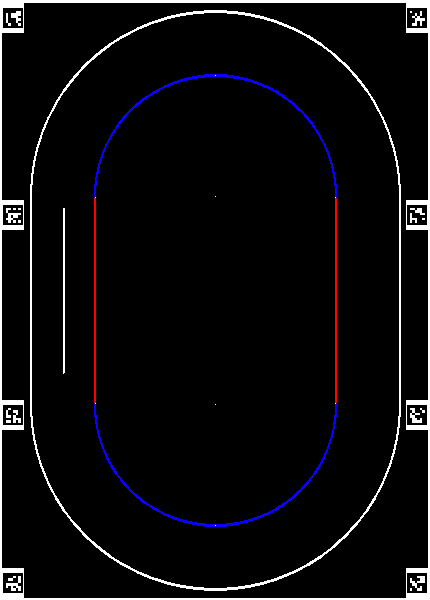
\includegraphics[scale=0.5]{pictures/map.png}
      \caption{Karte mit eingezeichneten Messpunkten.}
    \end{figure}
    \begin{itemize}
      \item{Linie links:} \( P_{1L} = (94, 197); P_{2L} = (94, 403) \) \\
        \( x = 94 \)
      \item{Linie rechts:} \( P_{1R} = (336, 197); P_{2R} = (336, 403) \) \\
        \( x = 336 \)
      \item{Kreis oben:} \( P_{CO} = (215, 196); r = 121 \) \\
        \( (x - 215)^2 + (y - 196)^2 = 121^2 \)
      \item{Kreis unten:} \( P_{CU} = (215, 404); r = 121 \) \\
        \( (x - 215)^2 + (y - 404)^2 = 121^2 \)
    \end{itemize}

  \section{Closest point on trajectory}
    Als erstes haben wir die gegebenen Koordinaten von Metern in Pixel umgerechnet, wobei \( 1m
    \equiv 100px \equiv 100cm \).

    Nun testen wir ob der angefragte Punkt einer der Mittelpunkte der Kreise ist. Sollte dies der
    Fall sein geben wir den Mittelpunkt auf dem halben Kreisbogen als Ergebnis zur"uck.

    Als n"achsten unterscheiden wir die 4 Quadranten der Karte: oberer Kreis, unterer Kreis, linke
    Linie, rechte Linie. Abh"angig vom Quadranten verwenden folgende Berechnung:
    \begin{itemize}
      \item{oberer Kreis:}
        \begin{eqnarray*}
          V & = & P - P_{CO} \\
          P_{closest} & = & \frac{P_{CO} + V}{|V| * r}
        \end{eqnarray*}
      \item{unterer Kreis:}
        \begin{eqnarray*}
          V & = & P - P_{CU} \\
          P_{closest} & = & \frac{P_{CU} + V}{|V| * r}
        \end{eqnarray*}
      \item{linke Linie:}
        \begin{eqnarray*}
          P_{closest} = (94, P.y)
        \end{eqnarray*}
      \item{rechte Linie:}
        \begin{eqnarray*}
          P_{closest} = (336, P.y)
        \end{eqnarray*}
    \end{itemize}
    Hierbei ist \( |V| \) die L"ange des Vektors. Quellcode:
    \url{https://github.com/bigzed/model_car/blob/version-4.0/texinput/src/closest_point_on_trajectory.py}

    \emph{Ergebnisse in \( px(cm) \):}
    \begin{itemize}
      \item{\((0,0)\)}: \( (125.58025288, 114.48246309) \)
      \item{\((200,400)\)}: \( (94, 400) \)
      \item{\((100,300)\)}: \( (94, 300) \)
      \item{\((200,215)\)}: \( (94, 215) \)
    \end{itemize}
    \begin{figure}[h]
      \centering
      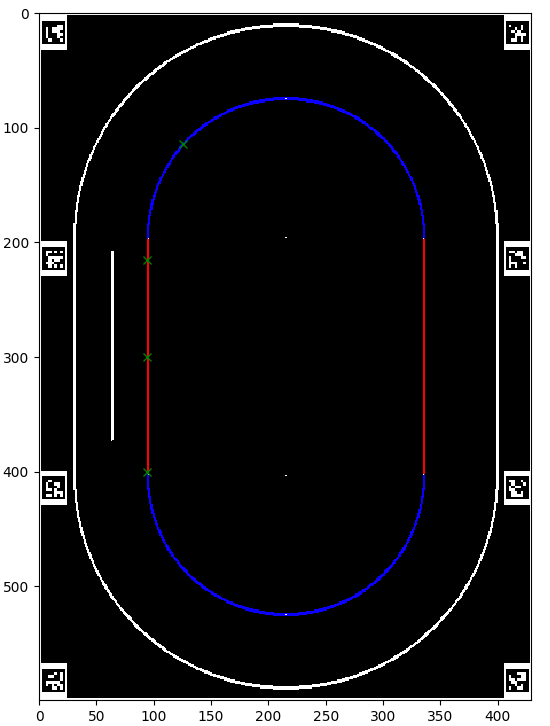
\includegraphics[scale=0.5]{pictures/closest_point_graph.png}
      \caption{Karte mit eingezeichneten n"achsten Punkten.}
    \end{figure}

  \section{Ceiling camera GPS}
\end{document}
